\documentclass{standalone}
\usepackage{amsmath}
\usepackage{tikz}

\begin{document}

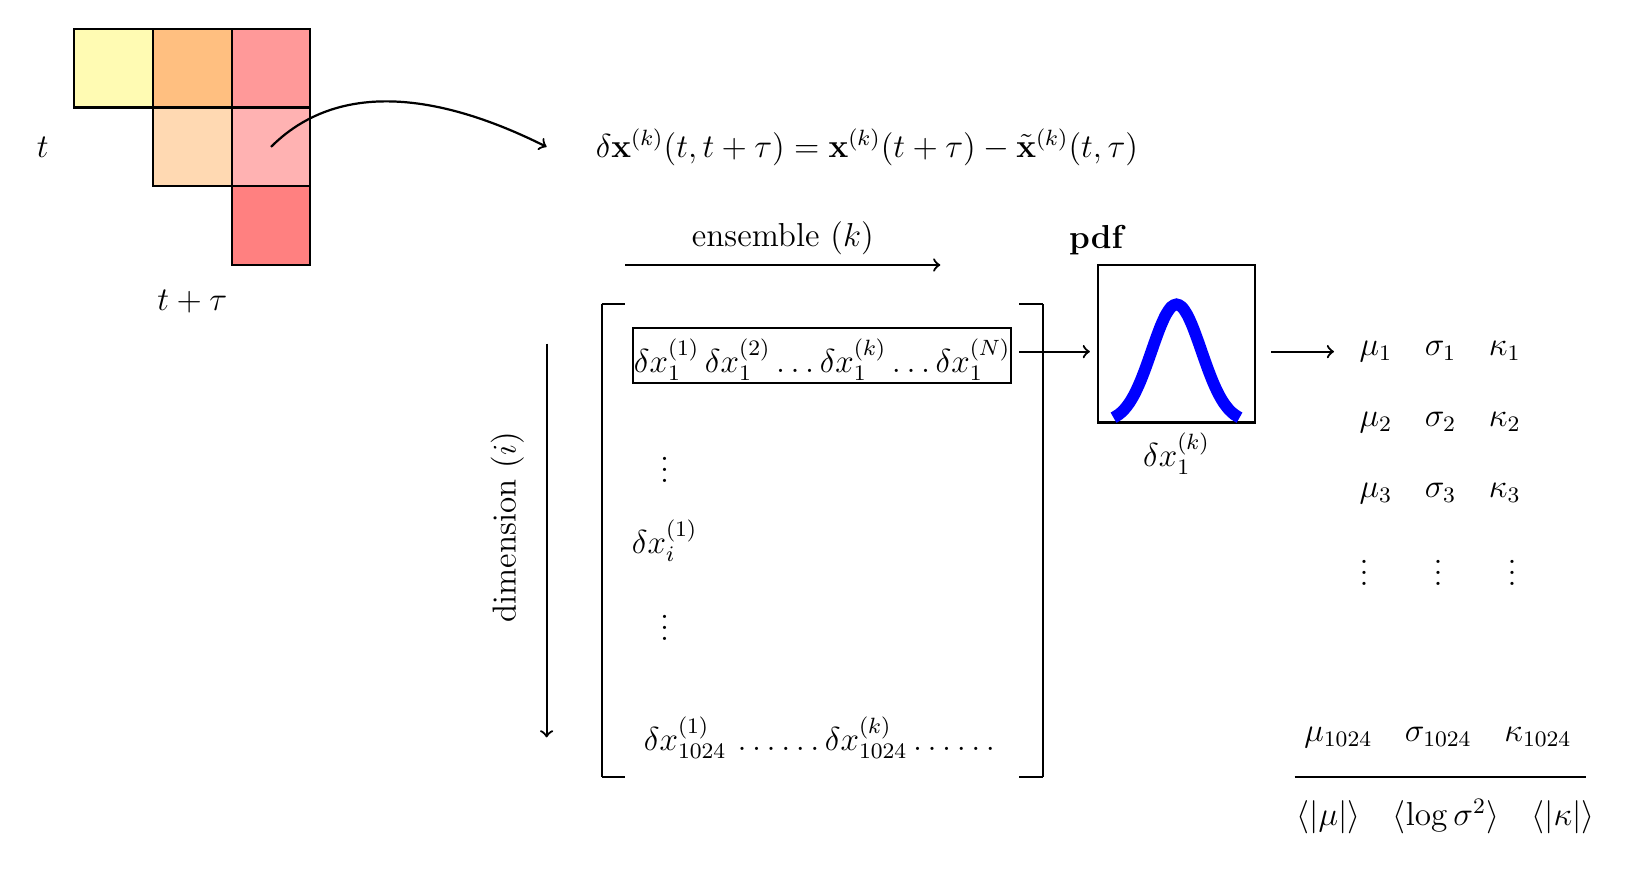
\begin{tikzpicture}
    % Draw the upper diagonal grid
    \draw[thick, fill=yellow!30] (0, 2) rectangle (1, 3);
    \draw[thick, fill=orange!30] (1, 1) rectangle (2, 2);
    \draw[thick, fill=red!50] (2, 0) rectangle (3, 1);
    \draw[thick, fill=orange!50] (1, 2) rectangle (2, 3);
    \draw[thick, fill=red!30] (2, 1) rectangle (3, 2);
    \draw[thick, fill=red!40] (2, 2) rectangle (3, 3);

    % Labels for t and t + tau
    \node[anchor=east] at (-0.2, 1.5) {\large $t$};
    \node[anchor=north] at (1.5, -0.2) {\large $t + \tau$};
    
    % Arrow pointing to the equation
    \draw[->, thick] (2.5, 1.5) .. controls (3.5, 2.5) and (5, 2) .. (6, 1.5);
    
    % Mathematical expression
    \node[anchor=west] at (6.5, 1.5) {\large $\delta \mathbf{x}^{(k)}(t, t+\tau) = \mathbf{x}^{(k)}(t+\tau) - \Tilde{\mathbf{x}}^{(k)}(t,\tau)$};

    \begin{scope}[shift={(7, -6)}]
        % Large matrix structure on the left
    % \draw[thick] (0, 0) -- (0, 5);  % Left vertical line
    % \draw[thick] (0, 5) -- (5, 5);  % Top horizontal line
    % \draw[thick] (5, 5) -- (5, 0);  % Right vertical line
    % \draw[thick] (0, 0) -- (5, 0);  % Bottom horizontal line

    % Opening bracket
    \draw[thick] (-0.3, 5.5) -- (-0.3, -0.5); % Large left bracket
    \draw[thick] (-0.3, 5.5) -- (0, 5.5); % Top horizontal
    \draw[thick] (-0.3, -0.5) -- (0, -0.5); % Bottom horizontal

    % Closing bracket
    \draw[thick] (5.3, 5.5) -- (5.3, -0.5); % Large right bracket
    \draw[thick] (5.3, 5.5) -- (5, 5.5); % Top horizontal
    \draw[thick] (5.3, -0.5) -- (5, -0.5); % Bottom horizontal

    % Rectangle with delta x terms inside the matrix
    \draw[thick] (0.1, 5.2) rectangle (4.9, 4.5);  % Rectangle for the delta x terms
    \node at (2.5, 4.8) {\large $\delta x_1^{(1)} \, \delta x_1^{(2)}  \ldots \delta x_1^{(k)} \ldots \delta x_1^{(N)}$};
    \node at (2.5, 0.0) {\large $\delta x_{1024}^{(1)} \, \dots  \ldots \delta x_{1024}^{(k)} \ldots \dots$};
    \node at (0.5, 3.5) {\large $\vdots$};
    \node at (0.5, 2.5) {\large $\delta x_i^{(1)}$};
    \node at (0.5, 1.5) {\large $\vdots$};

    % Arrow from rectangle to box
    \draw[->, thick] (5, 4.9) -- (5.9, 4.9);

    % Square box representing some operation or function
    \draw[thick] (6, 4) rectangle (8, 6);
    % Draw the bell curve inside the box
    \draw[line width=1.5mm, blue, domain=6.2:7.8, smooth, variable=\x] plot ({\x}, {4 + 1.5*exp(-(\x-7)^2/0.2)});
    \node at (7, 3.6) {\large $\delta x_1^{(k)}$};
    %\node at (6, 4.25) {\includegraphics[scale=0.3]{path/to/your/figure.png}};
    \node[anchor=south] at (6, 6) {\large \textbf{pdf}};

    % Arrow from box to the text labels
    \draw[->, thick] (8.2, 4.9) -- (9, 4.9);

    % Text labels (mu_1, sigma_1, kappa_1)
    \node[anchor=west] at (9.2, 4.9) {\large $\mu_1 \quad \sigma_1 \quad \kappa_1$};
    \node[anchor=west] at (9.2, 4) {\large $\mu_2 \quad \sigma_2 \quad \kappa_2$};
    \node[anchor=west] at (9.2, 3.1) {\large $\mu_3 \quad \sigma_3 \quad \kappa_3$};
    \node[anchor=west] at (9.2, 2.2) {\large $\vdots \quad \quad \vdots \quad \quad \vdots$};
    \node[anchor=west] at (8.5, 0.0) {\large $\mu_{1024} \quad \sigma_{1024} \quad \kappa_{1024}$};
    \node[anchor=west] at (8.4, -1.0) { \large $\langle |\mu| \rangle \quad \langle \log \sigma^2 \rangle \quad \langle |\kappa| \rangle$};

    \draw[-, thick] (8.5, -0.5) -- (12.2, -0.5);

    % Additional labels for dimension and ensemble
    \node[anchor=east, rotate=90] at (-1.5, 4) {\large dimension ($i$)};
    \draw[->, thick] (-1, 5) -- (-1, 0);
    \node[anchor=south] at (2, 6) {\large ensemble ($k$)};
    \draw[->, thick] (0, 6) -- (4, 6);

    \end{scope}

    
\end{tikzpicture}

\end{document}